In this section, we investigate how postulating various sorts of
\emph{introspection} may (or may not) lead to collapse results for \textsc{EviL}.

\subsubsection{Negative Doxastic Introspection}
We first recall the statement of negative doxastic introspection in
the single agent case:
\begin{equation*} 
\vdash \neg \Box \phi \to \Box \neg \Box \phi \label{dox-neg-intro}
\end{equation*}
It may be read, informally, as ``If the agent does not believe
some proposition $\phi$, then they believe that they do not believe
it.''  Given the justificatory nature of \textsc{EviL}, it is hard to
understand what this would be like.  What is the reason for believing
that you do not believe something?  Perhaps negative introspection 
comes from some kind of internal sensory apparatus.  We offer no
explanations for what might be this phenomenon, as we are admittedly
skeptical that it and find counter-intuitive.

As mentioned in \citep[\emph{Meditations II}]{vietch_descartes_2005},
it is plausible that, at any moment, one may try to cast just about
everything they know into doubt and reason from a minimal number of
assumptions.  We should assume, as Descartes, that these minimal
assumptions are \emph{safe}.  This philosophical insight is easily
expressed in as the following: \textsc{EviL}:
\begin{equation*} 
\DM\PP \label{descartes-posu}
\end{equation*}

However, together we can see that thinking about how these concepts
interact leads to a collapse of belief into truth for \textsc{EviL} Kripke structures:

\begin{theorem}[Negative Doxastic Collapse]\label{Doxastic-Collapse}
Consider any \textsc{EviL} Kripke structure $\mathbb{M}$ that makes
true doxastic negative introspection.  Then for all worlds $w$ and all
formulae $\phi$
\[ 
\mathbb{M}, w \Vdash \DM \PP \to \Box \phi \to \phi
\]
\end{theorem}
\begin{proof}
First assume $\mathbb{M}, w \Vdash \DM \PP$; if this does not hold then
the statement is vacuously true.  We must show $\mathbb{M}, w \Vdash
\Box \phi \to \phi$; by semantics it suffices to show that 
$$\mathbb{M}, w \Vdash \Box \phi \Longrightarrow \mathbb{M}, w \Vdash \phi.$$  
By our assumption know there must be some $v$ such that $w \sqsupseteq v$ and $\mathbb{M},v
\Vdash \PP$.  Thus $v R v$ from property \ref{pVII}, and from property
\ref{pVI} we may further conclude that
$v R w$.  Thus, we have:
\begin{equation*}
\mathbb{M},v \Vdash \Box \phi \Longrightarrow \mathbb{M},w \Vdash \phi 
\end{equation*}
Now assume that $\mathbb{M}, v \nVdash \Box
\phi$, then $\mathbb{M}, w \nVdash \Box \phi$.  This follows from
negative doxastic introspection, and may be observed in the following way:
\begin{align*}
\mathbb{M}, v \nVdash \Box \phi & 
 \Longrightarrow \mathbb{M}, v
\Vdash \neg \Box \phi \\
& \Longrightarrow \mathbb{M}, v
\Vdash \Box \neg \Box \phi & \textup{by negative doxastic introspection}\\
& \Longrightarrow \mathbb{M}, w \Vdash \neg \Box \phi & \textup{since
  $v R w$} \\
& \Longrightarrow \mathbb{M}, w \nVdash \Box \phi
\end{align*}
Contrapositively, this means that 
\begin{equation*}
\mathbb{M},w \Vdash \Box \phi \Longrightarrow \mathbb{M},v \Vdash \Box\phi 
\end{equation*}
Whence:
\begin{align*}
\mathbb{M}, w \Vdash \Box \phi & 
 \Longrightarrow \mathbb{M}, v
\Vdash \Box \phi \\
& \Longrightarrow \mathbb{M}, w
\Vdash \phi
\end{align*}
The above suffices to show the theorem.
\end{proof}

Informally, we may read Theorem \ref{Doxastic-Collapse} as asserting,
given doxastic introspection,
``If the agent knows anything, everything she believes is true.''  In
the concrete semantics, doxastic introspection has an even stronger
consequence:

\begin{theorem}[Concrete Collapse]\label{concrete-collapse}
Let $\Omega$ be an \textsc{EviL} model making true doxastic
introspection.  Then for all worlds $(a,A) \in \Omega$:
\[ \Omega, (a,A) \VDash \DM \PP \to \PP \]
\end{theorem}
\begin{proof}
It suffices to assume $\Omega, (a,A) \VDash \DM \PP$ and show $a
\models A$.  So fix some $\psi \in A$.

Since $\Omega$ can be understood as an \textsc{EviL} Kripke model via
(as we saw in Proposition \ref{evil_models} from \S\label{kipke}),
we know from Theorem \ref{Doxastic-Collapse} we have:
$$ \Omega, (a,A) \VDash \DM \PP \to \Box \phi \to \phi$$
Whence, by our assumption: 
$$ \Omega, (a,A) \VDash \Box \phi \to \phi$$

Since $\psi \in A$ we know that $\Omega,(a,A) \VDash \Box \psi$, hence
$\Omega,(a,A) \VDash \psi$.  Hence, by from Lemma \ref{truthiness},
the Truthiness Lemma from \S\ref{evil-grammar}, we have that $a
\models \psi$.

Since $\psi$ was arbitrary, we know that $a \models A$, as desired.
\end{proof}

While abstractly, we know that doxastic introspection implies a
collapse of belief into truth, concretely accessibility amounts to
truth.  We may read \ref{concrete-collapse} as asserting ``If the
agent has a sound argument, all of her arguments are sound.''


\subsubsection{Positive Doxastic Introspection}

While negative doxastic introspection leads to a serious collapse,
given the existence of a sound subset of the agents beliefs, no such
result obtains when postulating positive doxastic introspection.  A
rather simple example may be given using the concrete semantics:

\begin{proposition}
A \textsc{EviL} model with positive introspection does not necessarily
have the collapses seen in Theorem \ref{Doxastic-Collapse} and Theorem \ref{concrete-collapse}.
\end{proposition}
\begin{proof}
To show the proposition, we must exhibit a suitable counter-example.

Let $\Omega := \{(\varnothing, \varnothing), (\varnothing, \{\bot\})\}$.
This model is depicted in Fig. \ref{fig:counter-example}.  It is simple to
check that positive introspection holds, as the $R^\Omega$
accessibility relation is transitive.  Moreover, we can see that 
$$\mathfrak{M}, (\varnothing,
  \{\bot\}) \nVDash \DM\PP \to \Box \bot \to \bot$$
In a similar vain, we know that:
$$\mathfrak{M}, (\varnothing,
  \{\bot\}) \nVDash \DM\PP \to \PP$$
This means that it is not possible to prove either of 
the collapse theorems we previously saw.
\end{proof}
\begin{figure}[ht]
\centering
  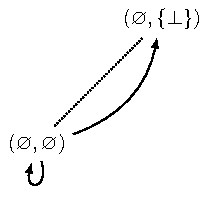
\includegraphics[]{evil_pictures/fifth_fig.pdf}
%\caption{A fairly simple example}
\caption{A model $\mathfrak{M}$ where $\mathfrak{M}, (\varnothing,
  \{\bot\}) \nVDash \DM\PP \to \Box \bot \to \bot$}
\label{fig:counter-example}
\end{figure}

Hence, with the above observation, we tentatively extend the
supposition that positive doxastic introspection may be construed as a
relatively safe addition to \textsc{EviL}, contrary to negative
doxastic introspection.

\subsubsection{Epistemic Introspection}

In this section we consider a positive and negative form of epistemic
introspection.  Unlike the case for doxastic introspection, we shall
reveal that neither of these assumptions are safe additions to \textsc{EviL}.

Recall the definition of knowledge proposed in \S\ref{soundness}; this
amounted to defining:
\[ K\phi := \DM(\PP \wedge \Box \phi)\]
This meant ``The agent has a sound argument.''  We might think of what
would happen if we assumed negative epistemic introspection using
this definition.  This would assert:
\[ \neg K \phi \to K \neg K \phi \]
Positive epistemic introspection can similarly be postulated as follows:
\[ K \phi \to K K \phi \]
Both forms of introspection have the following consequence:
\begin{theorem}
Assume that $\mathbb{M}$ is an \textsc{EviL} model which makes true
either \textbf{negative} introspection in the manner asserted above.  Then
for all formulae $\phi$ and all worlds $w$, we have:
\[ \mathbb{M}, w \Vdash \DM\PP \to \neg K \phi \to \BP \neg K \phi \]
\end{theorem}
\begin{proof}
Assume that  $\mathbb{M}, w \Vdash \DM\PP$, $\mathbb{M}, w \Vdash
\neg K \phi$, and assume $w \sqsubseteq v$.  We must show that $\mathbb{M}, v \Vdash \neg K \phi$.

We know the following:
\begin{bul}
\item From $\mathbb{M}, w \Vdash \DM\PP$, there is some $u \in P$ such
  that $u \sqsubseteq w \sqsubseteq v$.
\item We know that $u R u$ from property \ref{pVII}, and from property
  \ref{pVI} we have that $u R w$ and $u R v$
\item We know that $\mathbb{M}, u \Vdash \neg K \phi$.  For suppose
  towards a contradiction that
$\mathbb{M}, u \Vdash K \phi$, then there would be some $t \sqsubseteq
u$ such that $\mathbb{M}, t \Vdash \PP\wedge\Box \phi$.  However, by
transitivity (property \ref{pII}) we would have that $t \sqsubseteq
w$, whence $\mathbb{M}, u \Vdash \neg K \phi$, contrary to
our hypothesis. $\lightning$
\item From the above, we may gather:
\begin{align*}
\mathbb{M}, u \Vdash \neg K \phi & \Longrightarrow \mathbb{M}, u
\Vdash K \neg K \phi & \textup{by negative doxastic introspection} \\ 
& \Longrightarrow \mathbb{M}, u
\Vdash \Box \neg K \phi & \textup{since $\vdash K\phi \to \Box \phi$}
\\ 
& \Longrightarrow \mathbb{M}, v
\Vdash \neg K \phi & \textup{since $u R v$} \\ 
\end{align*}
\end{bul}
\end{proof}

\begin{theorem}
Assume that $\mathbb{M}$ is an \textsc{EviL} model which makes true
either \textbf{positive} epistemic introspection.  Then
for all formulae $\phi$ and all worlds $w$, we have:
\[ \mathbb{M}, w \Vdash \neg K \phi \to \BP \neg K \phi \]
\end{theorem}
\begin{proof}
 As before, assume that  $\mathbb{M}, w \Vdash
\neg K \phi$, and assume $w \sqsubseteq v$.  We must show that 
$\mathbb{M}, v \Vdash \neg K \phi$.

In this case we shall instead illustrate the result by
exhibiting the contrapositive, namely that if $\mathbb{M}, v \Vdash K \phi$ then $\mathbb{M}, w \Vdash K
\phi$.  Assuming $\mathbb{M}, v \Vdash K \phi$, then there is some $u
\sqsubseteq v$ such that $\mathbb{M}, u \Vdash \PP\wedge\Box \phi$.

Evidently, by the \textsc{EviL} properties \ref{pVI} and \ref{pVII} we
have that $u R w$.  Moreover, we know that 
\begin{align*}
\mathbb{M}, u \Vdash \PP\wedge\Box \phi & \Longrightarrow \mathbb{M},
u \Vdash \DM (\PP\wedge\Box \phi) & \textup{since $\sqsupseteq$ is
  reflexive} \\
& \Longrightarrow \mathbb{M},
u \Vdash K \phi & \\
& \Longrightarrow \mathbb{M},
u \Vdash K K \phi & \textup{by positive introspection} \\
& \Longrightarrow \mathbb{M},
u \Vdash \Box K \phi & \textup{since $\vdash K \phi \to \Box \phi$}\\
& \Longrightarrow \mathbb{M},
w \Vdash K \phi & \textup{since $u R w$}
\end{align*}
With the above, we have established what we set out to show.
\end{proof}

Before proceeding, we offer a way to read the above two theorems.

Negative epistemic introspection, for the proposed semantics for
knowledge, entails that ``If the agent knows anything at all, then if
she does not know something she never will.'' No matter what more
evidence she embraces, none of it will lead to sound arguments for
anything she does not already have sound arguments for, if she has any
knowledge at all.  In a way, negative doxastic introspection models
agents with ``enlightenment'' moments, where as they become more and
more aware of all of their evidence around them, they suddenly achieve
knowledge of some set of propositions, and then learn all that they
ever will.

The case for positive epistemic introspection is stronger than
negative introspection.  Given positive introspection, an agent can
never compose a sound argument by remembering certain details.
Knowledge, for any particular island, is completely static
(recall the definition of \emph{island} from \S\ref{islands}). Every
world in an island has exactly the same set of propositions for 
which the agent has a sound argument.  Positive epistemic
introspection, even more than negative epistemic introspection,
postulates that at any possible world, the agent cannot learn anything
by appealing to their own evidence. 

Hence, we should conclude that neither positive nor negative
epistemic introspection are particularly useful or intuitive axioms to
enforce on \textsc{EviL} models and Kripke structures.

%%% Local Variables: 
%%% mode: latex
%%% TeX-master: "evil_philosophy"
%%% End: 
